\documentclass{standalone}
\usepackage{tikz}
\usepackage{ctex,siunitx}
\setCJKmainfont{Noto Serif CJK SC}
\usepackage{tkz-euclide}
\usepackage{amsmath}
\usetikzlibrary{patterns, calc}
\usetikzlibrary {decorations.pathmorphing, decorations.pathreplacing, decorations.shapes,}

\begin{document}
\small
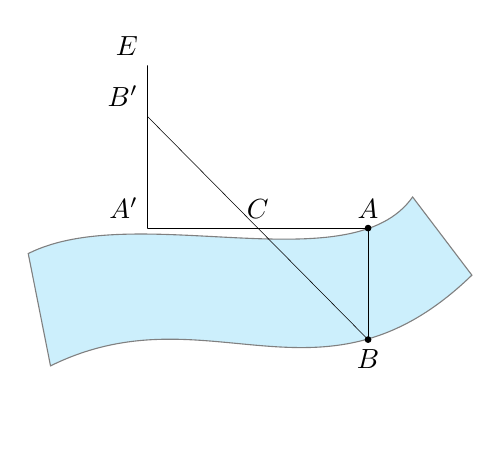
\begin{tikzpicture}[>=stealth,scale=0.8]
  \tkzSetUpPoint[fill=black]
  % \useasboundingbox(-1,-0.75)rectangle(3.7,1.4);
  \fill[cyan!20,draw=gray](-0.895, 2.016)..controls( 0.811, 2.874)and( 4.229, 1.524)..( 5.207, 2.914)--( 6.148, 1.673)..controls( 3.760,-0.640)and( 1.973, 1.471)..(-0.541, 0.233)--cycle;
  \tkzDefPoints{4.5/2.42/A,4.5/0.65/B,1.0/2.42/A',1.0/5.0/E}
  \tkzDefMidPoint(A,A')\tkzGetPoint{C}
  \tkzInterLL(B,C)(A',E)\tkzGetPoint{B'}
  \tkzDrawPoints(A,B)
  \tkzDrawSegments(A,B A',E B,B' A,A')
  \tkzLabelPoints(B)
  \tkzLabelPoints[above](A,C)
  \tkzLabelPoints[above left](A',B',E)
\end{tikzpicture}
\end{document}